\documentclass[12pt,titlepage]{article}
\usepackage[applemac]{inputenc}
\usepackage{amsmath}
\usepackage{amssymb}
\usepackage{graphicx}
\usepackage{subfigure}
\usepackage{multirow}
\usepackage[margin=.79in]{geometry}
\usepackage{caption}
\usepackage{url}

\begin{document}

\title{A BCI-Controlled Virtual Keyboard Design for Noisy Input and Limited Bandwidth} % Insert title
\author{Tamara Blain}
\maketitle

\begin{abstract}
This master's report addresses the problem of making BCI-controlled communication possible, given high classifier error-rate and extremely low bandwidth.

Brain computer interfaces (BCI) afford individuals with severe neuro-muscular impairments, direct neural control of external devices, with those enabling communication being among the most critical.  There are a variety approaches to the recording of brain activity, which can also serve as direct control and communication pathways from the brain to external devices.  We choose here to focus on electroencephalography (EEG)-controlled BCI.

Muscle contraction, eye movement, and even the heartbeat are a few sources of artifacts which lend to a noise in a scalp recorded EEG signal \cite{nunez_electric_2005}.  Amplitudes of EEG scalp recorded data are often on the order of microvolts, where amplitudes of artifacts such as those caused by eye movements, for example, can be on the order of millivolts \cite{tatum2007handbook}.  Thus, EEG signals are difficult to distinguish from artifacts \cite{nunez_electric_2005}.  In addition, EEG has fairly poor spatial resolution, and the tissue which makes up the brain conducts electrical signals from many 
different neuronal sources.  Add the fact that the desired signals are only a small sub scale of all 
brain activity, and the result is a very low signal to noise ratio.

Control of external devices requires that the BCI system be able to differentiate between different patterns in continuous brain signals \cite{lotte_review_2007}.  But currently, there remains a significant imbalance in bandwidths between a BCI system and its user.  Very little useful information is successfully extracted from an acquired neural signal, while feedback to the user can present a 
great deal of information.  Typically, the bit-rate of EEG-based BCI has been limited to around 0.5 bit/s \cite{millan2004}.  We consider a BCI system with the limitations imposed by an information transfer rate of $1$ bit $/$ $3$s (0.33bit/s).

The number of distinguishable patterns---\emph{brain states}---partially hinges upon classification 
accuracy \cite{lotte_review_2007}.  Information transfer rates (bit rates) decrease as accuracy decreases, potentially increasing the user's frustration and  undermining the viability of BCI as a widely used communication modality.  Therefore, low classification error is critical to the performance of BCI-controlled communication devices.  In order to enable effective communication in high error-rate environment, communication aids have to include ways of handling error, while optimizing the use of the available bandwidth.

We present a virtual keyboard, BinSpell, which is designed for noisy EEG signals leading to low-accuracy binary classifiers.  We use Huffman encoding techniques to more efficiently represent the user's intent as a series of binary choices.  We implement a language model to exploit the dependancies in language and infer intended symbols, in order to increase the rate of communication. Redundancy is used to counter the error rate of the classifier, and also help increase the communication rate.

The addition of redundancy to an already low-bandwidth environment, greatly reduced our rate 
of communication. But we use a language model to predict away as much of the redundancy 
inherent in language as we can, so that each choice the user makes provides the maximal 
amount of additional information.
\end{abstract}


\section{Introduction}

Many of the devices designed to make communication possible for individuals with motor 
disabilities require some vestige of neuro-muscular control.  Brain computer interfaces (BCI) 
affords individuals with severe neuro-muscular impairments direct neural control of external 
devices.  There are a variety of different methods for obtaining brain signals which are suitable 
for BCI control.  We choose here to focus on electroencephalography (EEG).  One of the 
primary objectives of BCI research has been to enable motor-limited individuals to control 
communication devices.  Thus, much research has gone into providing BCI-controlled spelling 
devices, or virtual keyboards, to these individuals.

Control of external devices requires that the BCI system be able to differentiate between 
different patterns in continuous brain signals \cite{lotte_review_2007}.  Muscle contraction, eye movement, and even the heartbeat are a few sources of artifacts which lend to a noise in a scalp recorded EEG signal \cite{nunez_electric_2005}.  Amplitudes of EEG scalp recorded data are often on the order of microvolts, where amplitudes of artifacts such as those caused by eye movements, for example, can be on the order of millivolts \cite{tatum2007handbook}.  Thus, EEG signals are difficult to distinguish from artifacts \cite{nunez_electric_2005}.  In addition, EEG has fairly poor spatial resolution, and the tissue which makes up the brain conducts electrical signals from many different neuronal sources.  Add the fact that the desired signals are only a small sub scale of all brain activity, and the result is a very low signal to noise ratio.

Currently, there remains a significant imbalance in bandwidths between a BCI system and its 
user. Very little useful information is successfully extracted from an acquired neural signal (for 
reasons explained briefly above), while feedback to the user can present a great deal of 
information.  Typically, the bit-rate of EEG-based BCI has been limited to around 0.5 bit/s \cite{millan2004}.  We consider a BCI system with the limitations imposed by a bit rate of 1 bit/3s (0.33bit/s).

The number of distinguishable patterns---\emph{brain states}---partially hinges upon classification 
accuracy \cite{lotte_review_2007}.  Information transfer rates (bit rates) decrease as accuracy decreases, potentially increasing the user's frustration and  undermining the viability of BCI as a widely used communication modality.  Figure \ref{fig:itrvsacc} displays the relationship between bit rate and accuracy.  Hence, low classification error is critical to the performance of BCI-controlled communication devices.  In order to enable effective communication in high error-rate environment, communication aids have to include ways of handling error, while optimizing the use of the available bandwidth.

One important design consideration is the compression of the maximal amount of information 
from the user, into the minimal number of bits.  Statistical properties of language can aid in this 
compression by providing context for compression algorithms.  While much work has gone 
into the improvement of classification methods, if one properly exploits the statistical 
properties of language, then one should be able to greatly improve effective rates of BCI 
enabled communication. 

Figure \ref{fig:BCI} illustrates how BCIs work with virtual keyboards controlled by binary input.  Typically, the user performs a mental activity which is dependent on the selection element they are trying to control \cite{molina_direct}.  The resulting brain signals are recorded via electrodes on the scalp, amplified and digitized \cite{lotte_review_2007}.  Classification algorithms identify features, or patterns, which correlate to certain identifiable brain events \cite{lotte_review_2007}.  Finally, these features are translated into a bit, which is sent to the keyboard, whose interface changes accordingly.

We present a virtual keyboard, BinSpell, which is designed for noisy EEG signals leading to low-accuracy binary classifiers.  We use Huffman encoding techniques to more efficiently represent the user's intent as a series of binary choices.  We implement a language model to exploit the dependancies in language and infer intended symbols, in order to increase the rate of communication. Redundancy is used to counter the error rate of the classifier, and also help increase the communication rate.

A second keyboard design presented, Circ-O-Spell, is an extension of an existing keyboard, 
Hex-O-Spell \cite{blankertz_advanced}.  With Circ-O-Spell, we present an alternative method of making selections, which we show requires fewer steps on average.  We also employ a Hidden Markov Model and 
borrow from Huffman coding such as to reduce the number of steps to a correct selection, and 
hence increase communication speed.  Circ-O-Spell provided us with the exploratory ideas 
which led to BinSpell.  Thus we focus primarily on BinSpell.

\begin{figure}[t]
\begin{center}
	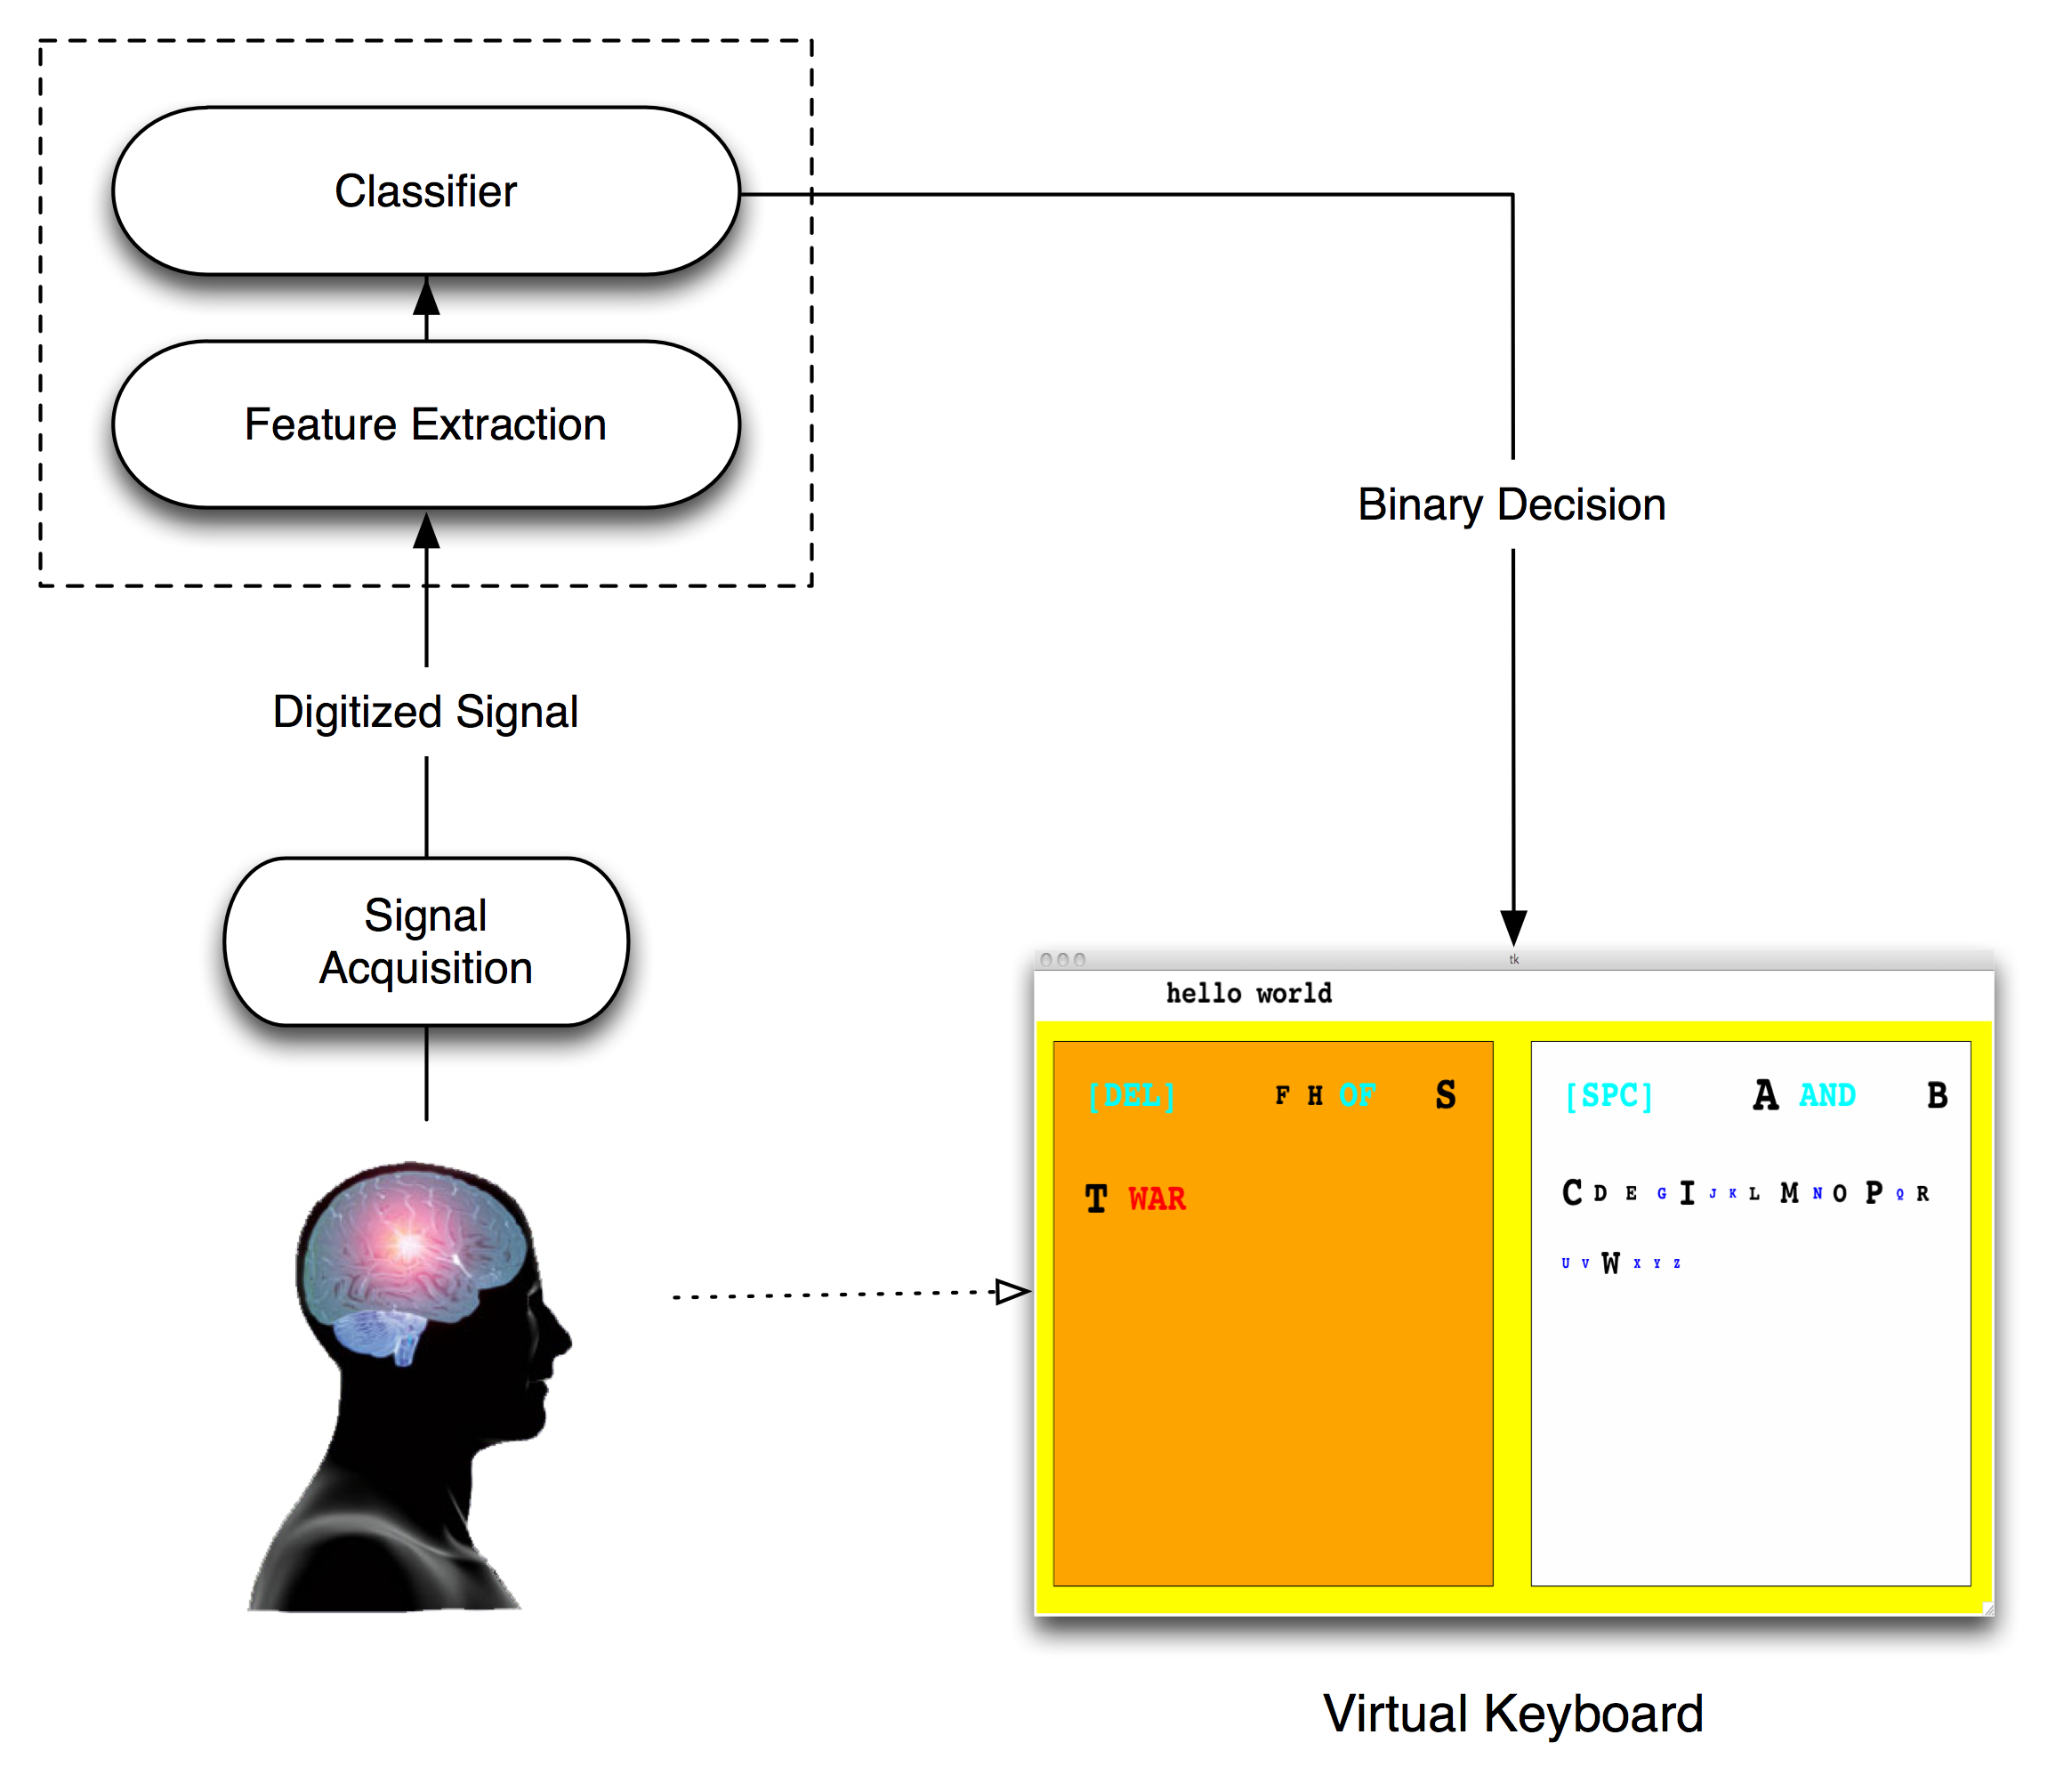
\includegraphics[scale=0.40]{Figure1.jpg}
	\captionof{figure}{BCI}
	\label{fig:BCI}
\end{center}
\end{figure}

\section{Background}

\subsection{Brain Imaging Techniques}

There are a variety approaches to the recording of brain activity, which can also serve as direct control 
and communication pathways from the brain to external devices.  Among them are 
electroencephalography (EEG), magnetoencepholography (MEG), positron emission tomography 
(PET), functional magnetic resonance imaging (fMRI), and near infrared spectroscopy (NIRS) [14].  EEG 
appears to be the most practical, commercially viable option thus far, due to its portability, and 
comparatively reasonable cost \cite{_next_????}.  The limitations of the remaining approaches are due mostly to the fact that they are technically demanding and expensive \cite{wolpaw_braincomputer_2002}.

\subsubsection{EEG}

Electroencephalography (EEG) uses electrodes which sit on the scalp, to measure voltage fluctuations 
in the brain.  The number of sensors used can range from 25 to 128 sensors.  Typically, a small area of 
the scalp is lightly abraded right before the application of a sensor.  This is done to reduce the 
impedance caused by dead skin cells.  A conductive gel is applied with each sensor, and each sensor is 
connected to a wire which feeds into an amplifier.  Scalp EEG is widely used in diagnosing many 
medical conditions such as epilepsy, strokes, and sleep disorders \cite{nunez_electric_2005}.  But translating those signals into meaningful information is very difficult.  One of the largest obstacles is the noise.

Single neurons are more complex than even the most sophisticated neural networks, and brain 
processes often involve their interactions at multiple scales \cite{nunez_electric_2005}.   EEG has inherently low spatial 
resolution, so the signals picked up from EEG  sensors reflect the activity of millions of neurons \cite{nunez_electric_2005}.  In 
addition to brain activity, electrical signals from the scalp can also come from sources such as eye 
blinks or tongue movement \cite{nunez_electric_2005}.  Electrical impulses from the heart can actually produce scalp potentials 
greater than EEG amplitudes \cite{nunez_electric_2005}, thus making recorded signals even more difficult to discriminate. 
Additionally, the electrical and geometrical properties of the brain itself, as well as the skull and scalp, 
all lend to the quality of recorded signals \cite{nunez_electric_2005}.  All of these factors contribute to the extremely low signal 
to noise ratios in recorded signals.


\subsection{BCI}

\begin{table}
\caption{Comparison of typing speeds achieved by existing virtual keyboards.}
\begin{center}
\begin{tabular}{lllll}
\hline\hline
& Hex-O-Spell & P300 & P300 & Dasher\\
\hline
Classifier & \multirow{2}{*}{LDA} & Stepwise & \multirow{2}{*}{SVM} & Classification \\
\quad (accuracy $>$ 90\%) & & LDA  & & Matrix \\
Average spelling rate & \multirow{2}{*}{$4.24$} & \multirow{2}{*}{$\sim4$} & \multirow{2}{*}{$11.1$} & \multirow{2}{*}{$\sim5.6$} \\
\quad (chars/min) & & & & \\
Achieved spelling & \multirow{2}{*}{$2.3$--$7.6$} & $2.8$--$7.8$ & \multirow{2}{*}{$6.67$--$16.7$} & $3.2$--$14.4$ \\
\quad rates (chars/min) & & (offline testing) & & (Avg.) \\
\hline\hline
\end{tabular}
\end{center}
\label{table:BCIComp}
\end{table}

A brain computer interface (BCI) is a communication channel between the brain and a 
computer (figure~\ref{fig:BCI}). It records changes in electrical activity in the brain, and translates them into 
control signals.  Acquired signals are first amplified, then digitized for analysis.  Unwanted 
artifacts, such as those produced by a heartbeat, and eye blinks, are filtered out, and the target signal
feature is extracted \cite{lotte_review_2007}.   Built-in classifiers characterize brain state by correlating specific mental 
activities with the target features \cite{lotte_review_2007}.  The interpreted brain state is commuted into control signals (a single bit in our case), and sent to the device being operated.

BCI's can be either invasive, such as single-unit recording or electrocorticography (EcoG), or 
non-invasive, such as EEG or MEG.  Invasive techniques provide the most information per 
channel, but carry the greatest risk, as they require surgery to provide openings in the skull. 
Most BCI systems are non-invasive, and use EEG signals recorded from the scalp \cite{guger_design_1999}.

\subsection{Virtual Keyboards} % Incomplete

Generally, virtual keyboards are devices or software, which emulate physical keyboards, but do 
not have physical sensing buttons \cite{kolsch2002keyboards}.  They are often controlled by pointing devices, such as mice, 
touch pads, photo-electric sensing devices, or active finger tracking methods \cite{kolsch2002keyboards}.  Virtual 
keyboard key layout can be dynamic, and can readily include words, phrases, or pictures.  Virtual keyboards designed for BCI control are on-screen keyboards.  Although the area of 
software keyboards is limited by the size of the screen on which it is displayed, they can be 
more adaptable to compact mobile devices.

\section{Related Work}

\subsection{P300 Speller}

\begin{figure}[t]
\begin{center}
	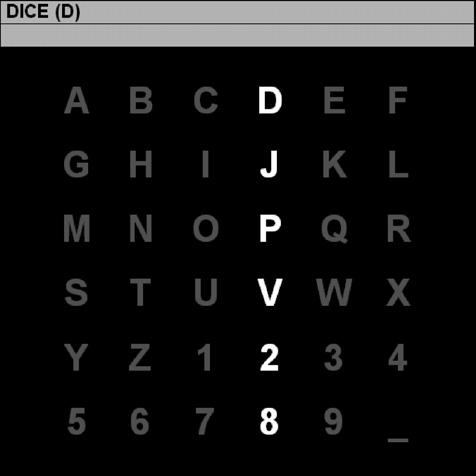
\includegraphics[scale=0.40]{Figure2.jpeg}
	\captionof{figure}{P300 Speller}
	\label{fig:P300}
\end{center}
\end{figure}

The P300 Speller is an synchronous EEG controlled spelling system.   It relies on the P300 event 
related potentials (ERPs) that result when users respond to specific stimuli generated by the BCI 
system \cite{sellers_p300-based_2006}.  In this paradigm (shown in figure~\ref{fig:P300}), users are presented with a $6\times6$ matrix of symbols, where 
each cell contains a symbol \cite{sellers_p300-based_2006}.  The user is asked to focus on their symbol of choice.  The rows and 
columns are flashed randomly, until the appropriate response signal is detected \cite{sellers_p300-based_2006}.  The desired output
is the intersection of the row and column which elicits the P300 signal \cite{sellers_p300-based_2006}.

Although it requires the use of signal averaging, as the random sequence stimuli have to be presented 
multiple times, research into improving P300 classification rates has resulted in reported typing rates 
between $2.8$ and $7.8$~chars/min \cite{sellers_braincomputer_2004}.  Some classification techniques promise substantial increases in 
P300 typing speed, of up to $16.67$~chars/min \cite{wolpaw_braincomputer_2002}.  Improvements to the P300 Speller have focused mainly on improvement of classification algorithms designed to detect P300 signals \cite{krusienski2006comparison} \cite{wolpaw_braincomputer_2002} \cite{sellers_braincomputer_2004}.

\subsection{Hex-O-Spell}

\begin{figure}[t]
\begin{center}
	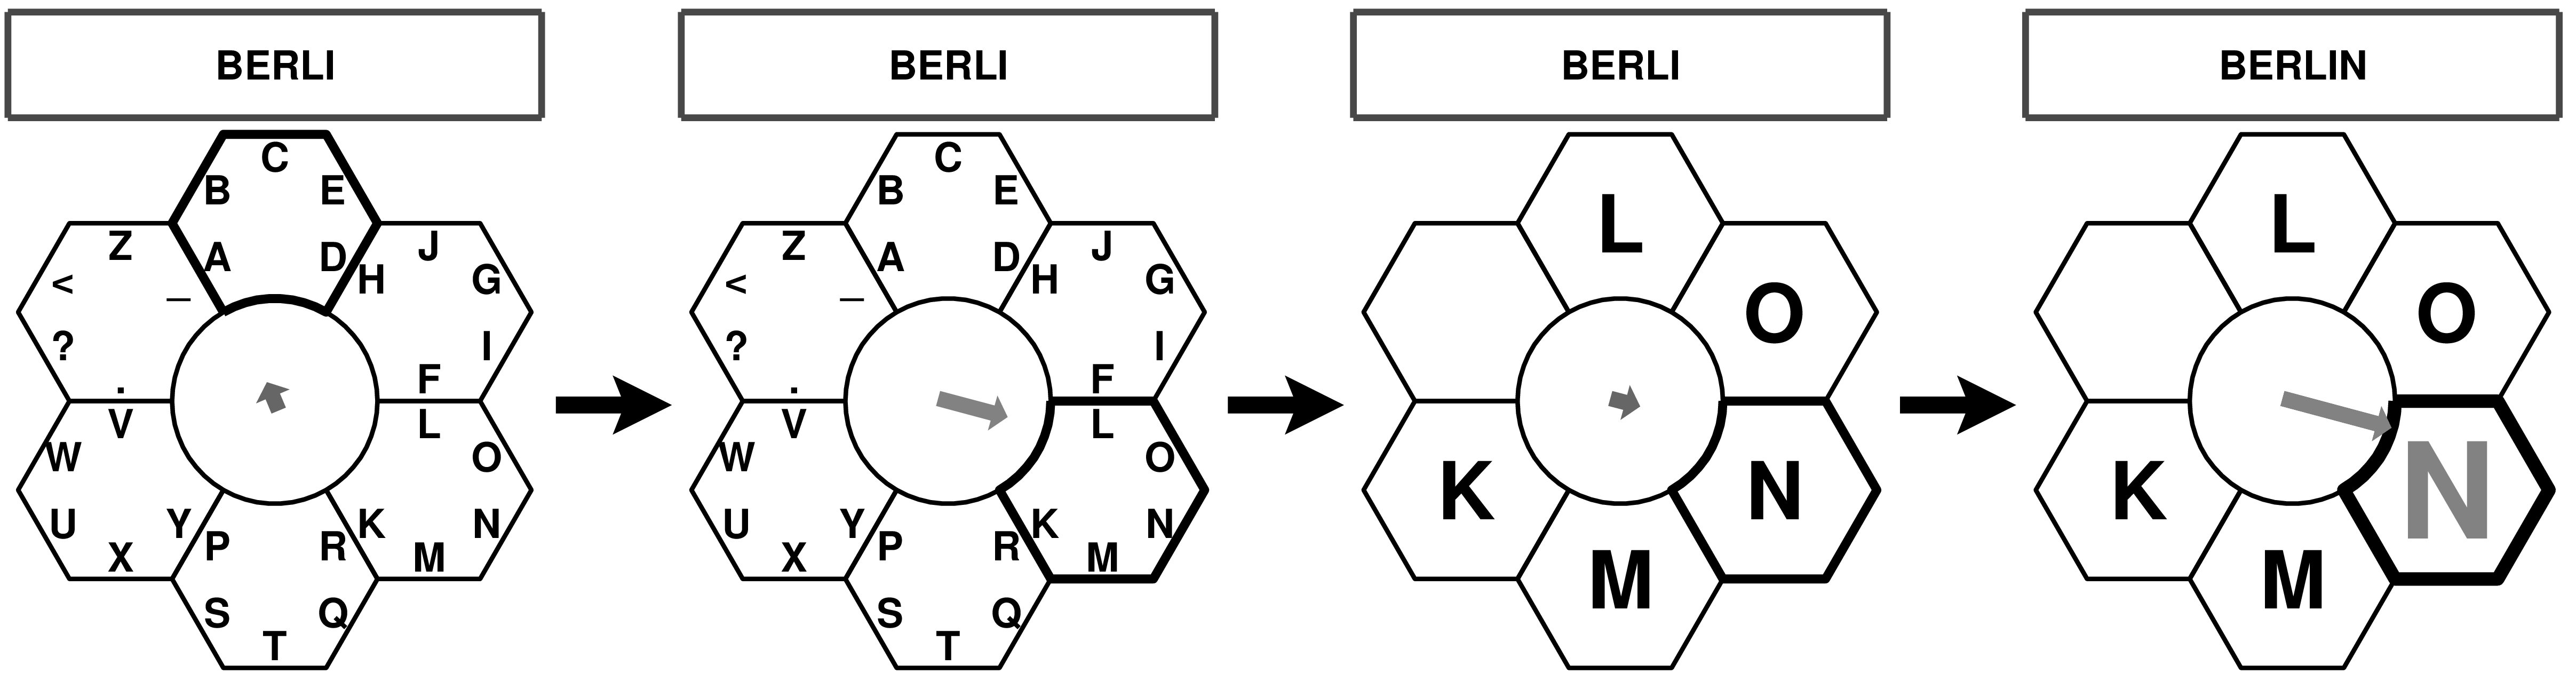
\includegraphics[scale=0.10]{figure3.jpeg}
	\captionof{figure}{Hex-O-Spell}
	\label{fig:Hex}
\end{center}
\end{figure}

Hex-O-Spell keyboard layout is comprised of $6$ hexagonal fields surrounding a circle, each containing 
$5$ characters (figure~\ref{fig:Hex}).  The center of the circle contains an arrow used to make selections.  A language 
model determines how the letters are arranged within each hexagon \cite{blankertz_berlin_2006}.

Hex-O-Spell is mentally controlled by imagined right hand and foot movements \cite{blankertz_advanced}.  Imagined right 
hand movement effects a clockwise rotation of the arrow in the center of the circle.  Imagined right foot 
movement ceases rotation, and causes the arrow to extend towards a hexagon \cite{williamson_designing_2009}.  Selection of a 
hexagon is caused by sustained right foot motor imagery, and causes all other hexagons to be 
cleared \cite{williamson_designing_2009}.  The 5 characters in the chosen hexagon are then redistributed among the empty hexagons, 
and the arrow is reset to its minimal length \cite{williamson_designing_2009}.  Parameters such as the arrow turning and growing 
speeds can be tailored to the user.

Hex-O-Spell is controlled by the Berlin Brain Computer Interface (BBCI), an EEG-based
system which decodes motor imagery without subject training \cite{schalk_bci2000:general-purpose_2004}.  Much of the  focus 
concerning the improvement of Hex-O-Spell, has been on the improvement of the front end.  The 
relationship between control, action, and belief were considered in its design, as was the ``cost'' of an 
action \cite{williamson_designing_2009}.  It The language model used by Hex, its use of machine learning techniques and its ability to 
operate at high decision speeds, affords high quality feedback to the user \cite{blankertz_advanced}. \cite{blankertz_advanced} reports 98\% accuracy at 
an average speed of $1$~decision every  $2.1$~s and a peak ITR of $22.1$ bits/s.

Hex-O-Spell was tested with two subjects who had no training on the BBCI, and who had very little 
experience with the keyboard \cite{blankertz_berlin_2006}.  The achieved typing speeds were between $2.3$ and $5$ chars/min for 
one subject, and between $4.6$ and $7.6$ char/min for the other, for error-free completed phrases \cite{blankertz_berlin_2006}.

\subsection{Dasher}

Dasher is a zooming interface (figure~\ref{fig:Dash}) which uses a language model to predict the probabilities of 
symbols given a context, and determine the size of the symbols based on those probabilities.  So the 
letters with the largest probabilities given the output text will be more easily seleccted.  When the 
predictions are correct, sequences of letters can be chosen quickly with a continous gesture.

Dasher was designed as an alternative to the standard keyboard, and designed to be used with any input 
methods.  It uses a sextuplet-gram language model to accurately predict letters contextually \cite{mackay_dasherefficient_2003}. The 
language model can be trained on any text, making it biased towards the set of words and phrases the 
user is most likely to use \cite{wills_dasher-efficient_2006}.  With error-free, binary input, Dasher can emit text at a rate of $1$ character 
every $1$ bits \cite{mackay_dasherefficient_2003}.  Spelling rates of up to $14.4$ chars/min have been reported with BCI-controlled Dasher \cite{felton2007neural}, 
with an average of $\sim5.6$ chars/min.

\section{Our Approach}

\begin{figure}[t]
\begin{center}
	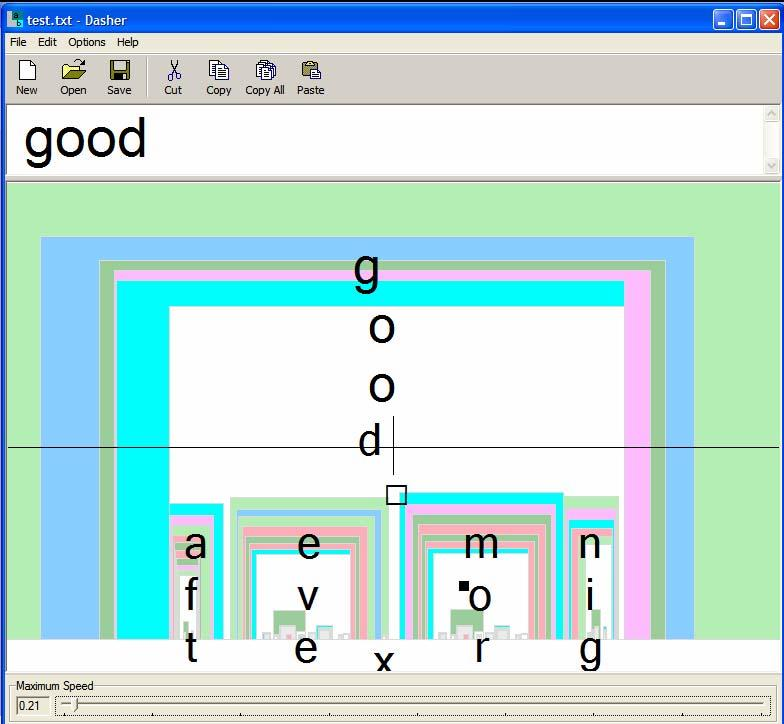
\includegraphics[scale=0.25]{figure4.jpeg}
	\captionof{figure}{Dasher}
	\label{fig:Dash}
\end{center}
\end{figure}

\subsection{Circ-O-Spell}

\subsubsection{Design and Operation}

This keyboard is an extension of the Hex-O-Spell keyboard [31].  The hexagonal fields are replaced by 
circular fields, containing sets of symbols (figure~\ref{fig:CircA}).  Circ-O-Spell is intended to be controlled by the 
output of a binary classifier.  State-0 brings about rotation and state-1 achieves selection.  When a circle 
containing a set of symbols is selected, a new layout is presented containing only the symbols in the 
selected set (figure~\ref{fig:CircC}).  In this new layout, each symbol from the selected set gets its own circle, and 
symbols for `back-space' and delete are also presented.  Delete removes the most recently output 
symbol from the text box, exits the new layout, and returns the keyboard to the state prior to the 
selection of that symbol.  The back-space key exits the new layout, and returns the user to the layout 
immediately preceding entrance into the new layout.  If the selected circle contains only one symbol, 
that symbol is added to the text box at the top of the window, and the user is returned to a layout where 
all the letters are presented (figure~\ref{fig:CircD}).

\subsubsection*{Implementation Details}

Letter and word frequencies are an important consideration when designing a system for the purpose of 
enabling communication \cite{jones_case-sensitive_2004}.  They can be used to calculate probabilities which help capture important 
properties of language, and allow for prediction of a letter, word, or phrase in a speech sequence \cite{jones_case-sensitive_2004}.  n- 
grams are groups of letters, words, or phrases of size~$n$, which serve as the basis for many probabilistic 
language models \cite{reviewer-lee_review_2000}.  n-grams do have shortcomings in that they can only capture dependencies within 
their own length \cite{reviewer-lee_review_2000}.  They cannot explicitly represent any long range dependencies and are thus unable 
to distinguish them from noise \cite{reviewer-lee_review_2000}.

Higher order $n$-grams can provide more information, as they reflect the frequencies of larger units \cite{jones_case-sensitive_2004} 
but tend to introduce more sparsity \cite{_url.ppt_????}.  This sparsity can be resolved, however, with large corpora, 
smoothing techniques, and the incorporation of contextual information \cite{curran_very_2002}, \cite{russell_artificial_2002}.  \cite{rawlinson_bigram_1976} argues that most letter-level
bigram frequency tables reflect unrealistic counts because they do not use the positions of  those 
bigrams within words as contextual information.  They demonstrate a marked difference in letter 
bigram frequencies, depending on their positions within words \cite{rawlinson_bigram_1976}.

\begin{figure}[t]
\centering
\subfigure[]{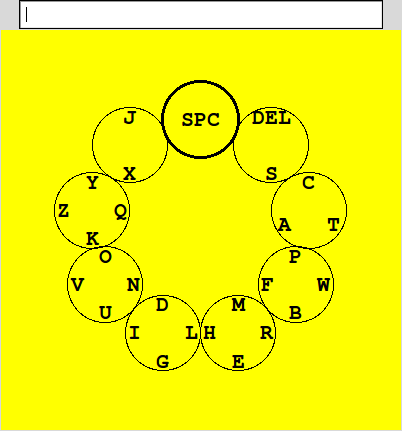
\includegraphics[scale=0.30]{fig4.png}\label{fig:CircA}}
\subfigure[]{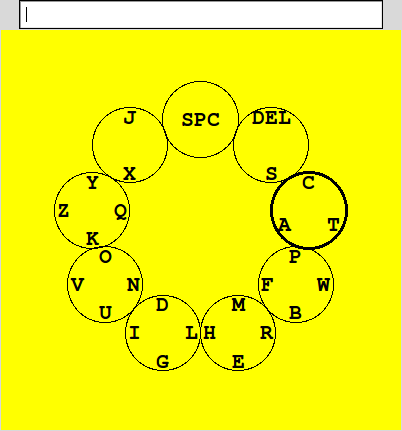
\includegraphics[scale=0.30]{fig5.png}\label{fig:CircB}}
\subfigure[]{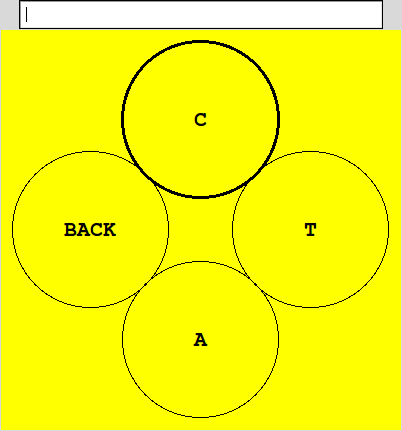
\includegraphics[scale=0.30]{fig6.png}\label{fig:CircC}}
\subfigure[]{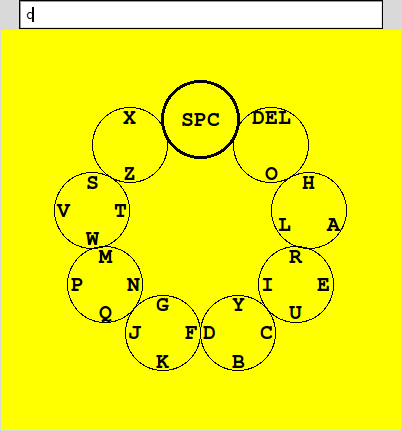
\includegraphics[scale=0.30]{fig7.png}\label{fig:CircD}}
\caption{Circ-O-Spell}
\end{figure}

Markov models are models of probabilistic temporal processes, which satisfy the Markov assumption---that
is, the current state depends only on a finite history of previous states \cite{russell_artificial_2002}.  The order of a Markov 
process defines the number of previous states on which the current state is Dependent.  The simplest is 
the first-order Markov process, which assume that the current state is dependant only on the previous 
state, not any other earlier states \cite{russell_artificial_2002}.  First-order Markov processes are characterized by their prior
probabilities, transition models, and emission models.  Borrowing notation from \cite{russell_artificial_2002}, where $X_t$  denotes
a state variable at time $t$, prior probabilities $P(X_.)$ define the probabilities over the states at the first 
time step.  The transition model is a conditional distribution $P(X_t | X_{t?1})$  describing how the state 
evolves over time.  The observation model is also a conditional distribution $P(E_t | X_t)$ which describes 
the probabilities on the evidence variables $E_t$ , the output, at every time step.  Markov models often 
make up the formalism behind $n$-gram models used in natural language processing \cite{brown_class-based_1992}, \cite{makhoul_state_1995}. 
Circ-O-Spell uses a first-order Markov Model to attempt to reduce the number of steps needed to make 
a selection.  We describe our calculations below and use the notation in Table~\ref{table:Not}.

\begin{gather*}
P(X_0 = x_i) = \frac{\displaystyle C_1(x_i x_j)}{\displaystyle \sum_{i=1}^k \sum_{j=1}^k C_1(x_i x_j)} \tag{1} \\
P(X_1 = x_j | X_0 = x_i) = \frac{\displaystyle C_1(x_i x_j)}{\displaystyle C_1(x_i)} \tag{2} \\
P(X_t = x_j | X_{t-1} = x_i) = \frac{\displaystyle C_2(x_i x_j)}{\displaystyle C_2(x_i)} \tag{3}
\end{gather*}

The default letter layout is determined by the order of the probabilities calculated by Equation (1). 
When a circle-set containing the letter of choice is selected, the letter with the highest probability 
among that set, is highlighted in the next layout to facilitate faster selection.  The arrangement of the letters, after a single 
letter is output into the text box, is determined by Equation (2).  Equation (3) describes the conditional 
probabilities for each letter in any states which follow.  The frequency tables from which the counts are obtained, represent bigram frequencies per $1000$ 
words, of words occurring at least once per million in normal usage, and of more than three letters \cite{rawlinson_bigram_1976}.

\subsection{BinSpell}

\subsubsection{Design and Operation}

\begin{table}
\caption{Explanation of notation.}
\begin{center}
\begin{tabular}{ll}
\hline\hline
$X_t$ & State variable at time $t$ \\
$C_1(.)$ & Count of bigrams found solely and the beginning of a word \\
$C_2(.)$ & Count of bigrams found at any other position in a word \\
$x_i$ & Letter of the alphabet \\
$C_1^W(.)$ & Word-level unigram counts \\
$C_2^W(.)$ & Word-level bigram counts \\
$W_t$ & State variable in word-level Markov process \\
$w_i$ & A single word \\
$C_3^X(.)$ & Letter-level trigram counts \\
\hline\hline
\end{tabular}
\end{center}
\label{table:Not}
\end{table}

BinSpell (Figure~\ref{fig:BinA}) is also designed to be controlled by the output of a binary classifier.  State 0 causes 
selection of the box on the left and state 1 selects the box on the right.  The user is intended to select the 
box with the symbol of their choice.  Symbols offered include single characters, space, delete, and 
whole words.  The symbols for space and delete are not offered, however, until at least one other 
symbol has been typed.  The size and color of symbols are determined by their probabilities, the 
computation of which we explain later.  Symbols with the lowest probabilities are small and blue, the 
next largest are black.  The most likely symbol is the largest and is displayed in red.  Whole words are 
provided in cyan to help distinguish them from single letters.  Selection of a box causes all of the 
symbols to be reordered and redistributed between the boxes (Figure~\ref{fig:BinB}).  This selection process is repeated 
until one of the probabilities surpasses a threshold (Figure~\ref{fig:BinD}), and the associated symbol is output into the text box 
at the top (Figure~\ref{fig:BinD}). 

\subsubsection{Implementation Details}

\begin{figure}
\centering
\subfigure[]{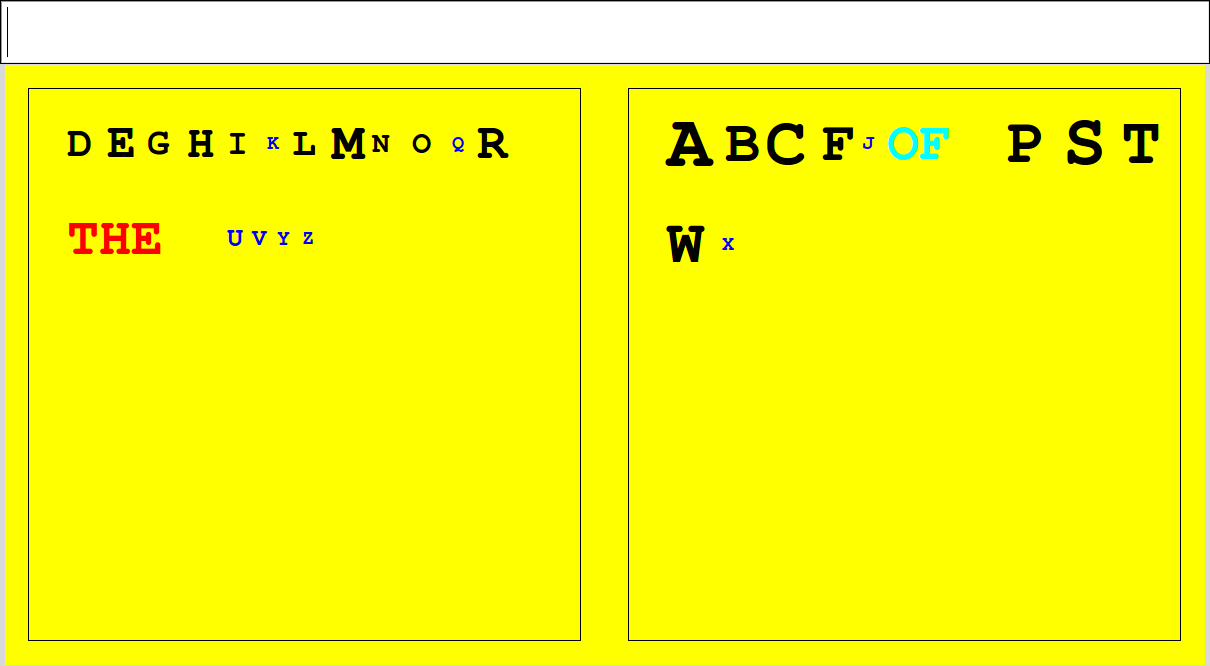
\includegraphics[width=.4\textwidth]{fig8.png}\label{fig:BinA}}
\subfigure[]{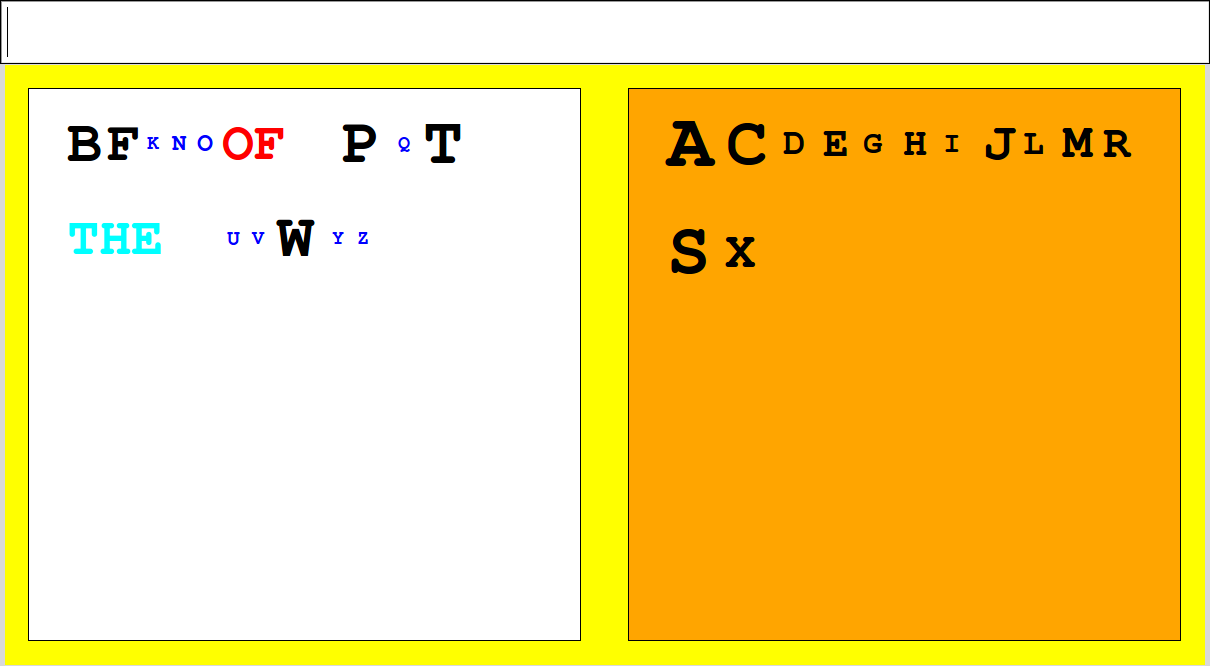
\includegraphics[width=.4\textwidth]{fig9.png}\label{fig:BinB}}
\subfigure[]{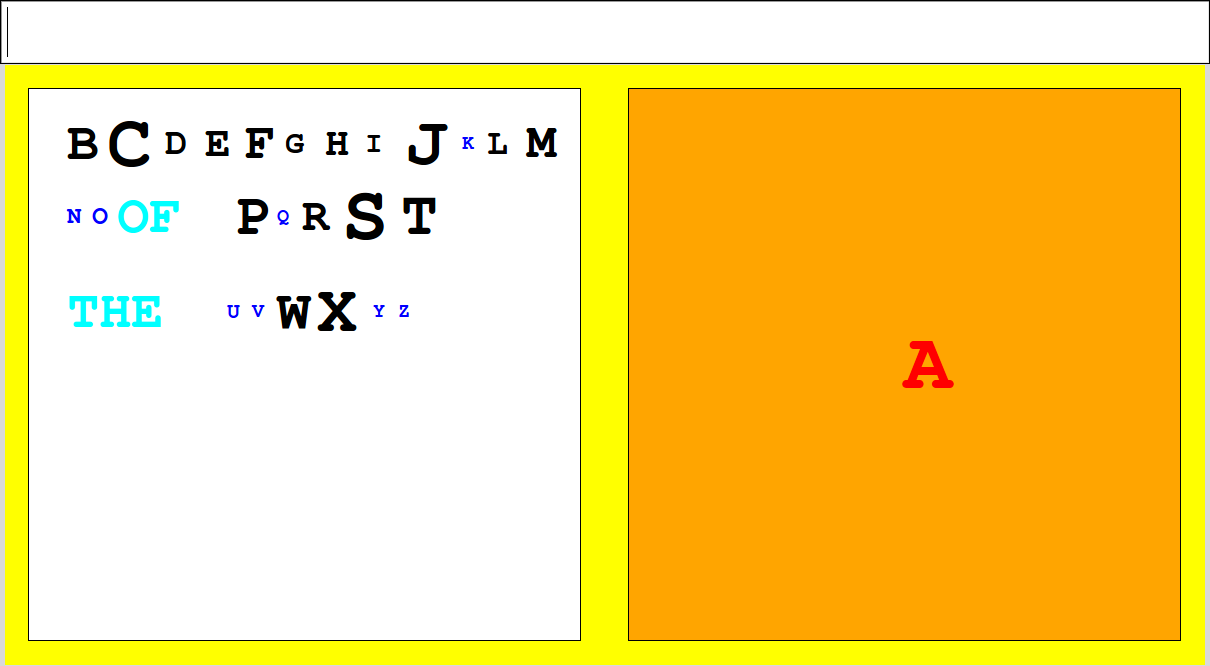
\includegraphics[width=.4\textwidth]{binA.png}\label{fig:BinC}}
\subfigure[]{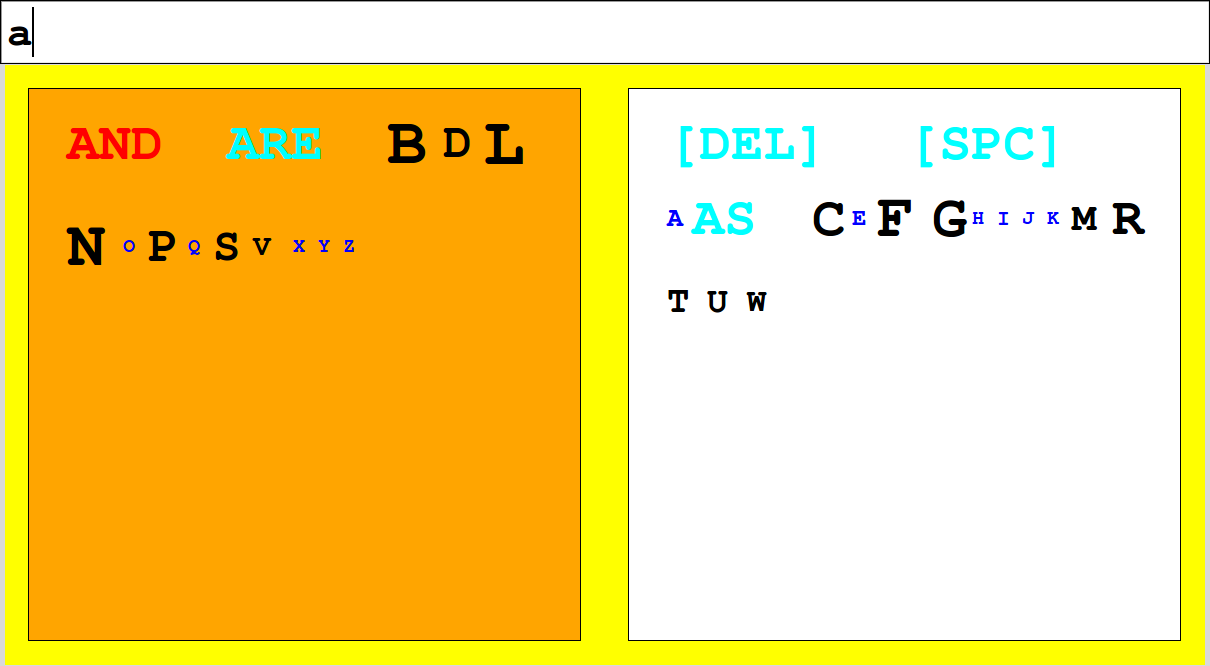
\includegraphics[width=.4\textwidth]{fig10.png}\label{fig:BinD}}
\caption{BinSpell}
\label{fig:Bin}
\end{figure}

Huffman coding is an algorithm originally designed for the binary encoding of sequences of ASCII 
symbols.  It uses each symbol's frequency of occurrence to build up an optimal way of representing that 
character as a binary string \cite{cormen_introduction_2001}.  It works by creating a binary tree of nodes, each of which represents a 
symbol and it's associated probability. The way in which the tree is walked produces codes that 
represent the symbols.  Thus the least number of bits encode the most commonly used symbols.  It is 
most commonly used within lossless compression schemes, such as JPEG, or MP3 \cite{cormen_introduction_2001}.

We use Huffman coding to determine the members of a box-set,  reducing the number of steps it would 
take to access the most likely symbols.  Thus, the left and right boxes reflect loosely the left and right 
halves of a Huffman tree, and the selection process is based on a Huffman-coded decision tree.  Individual letters within a box are alphabetized, however, to facilitate visual scanning.

When a selection is made, the probabilities of all symbols within that box are weighted by the accuracy 
of the classifier (80\% in our case).  The probabilities of the symbols in the box that was not chosen are 
weighted by one minus the accuracy.  All of the probabilities are then re-normalized, and a new 
Huffman tree is generated and used to determine the new layout.  The flowchart representing this 
process can be seen in Figure~\ref{fig:BinFlow}.

Selections also cause the background of the selected box to be shaded in orange, while the background 
color of the non-selected box becomes white (Figure~\ref{fig:BinB}).  If a box is selected in succession, the border of the 
box is intensified for a few seconds, in order to indicate its selection.  Selection of a word outputs the 
word into the text box.  As a policy, a space character is automatically appended to a whole word 
selected.  The selection of delete following an incorrectly selected word causes the entire word to be 
erased.  Then both the text box and the keyboard are returned to the state prior to the incorrect 
selection.

BinSpell implements a 2\textsuperscript{nd}-order, character-level Markov process in parallel with a 1\textsuperscript{st}-order, word-level 
Markov process, as its language model.  First-order Markov processes are explained in the previous 
section.  Second-order Markov processes assume the current state depends only on the previous two 
states, and no other history.  We calculate prior probabilities, transition probabilities, and output 
probabilities for both processes and describe them below (notation is in Table~\ref{table:Not}).
\begin{gather*}
P(W_0 = w_i) = \frac{C_1^W(w_i)}{\displaystyle \sum_{j=1}^n C_1^W(w_j)} \tag{4} \\
P(W_t = w_j | W_{t-1} = w_i) = \frac{C_2^W(w_i w_j)}{\displaystyle C_2^W(w_i)} \tag{5} \\
P(X_t = x_k | X_{t-1} = x_j, X_{t-2} = x_i) = \frac{C_3^X(x_i x_j x_k)}{\displaystyle C_3^X(x_i x_j)} \tag{6}
\end{gather*}

Priors at the letter-level are calculated as in Equation (1), utilizing the same bigram frequency counts 
used in Circ-O-Spell.  Word-level unigram counts determine prior probabilities for each word 
as in Equation (4).  In designing BinSpell, we had to make a choice about how to weigh letter-level and 
word-level probabilities relative to one another.  For lack of information on how to optimally make this 
choice, we assigned them equal weight, and put off further investigation of this question, to a future 
date.  We chose to restrict the number of words presented to the user to 3, and we explain their 
selection below.  Next, the priors of all the letters and words presented are renormalized.  Finally, 
Huffman coding determines in which box they will be displayed conditional probabilities which 
determine the state transitions at both levels are calculated after a single symbol has been output.  At 
the letter level, the distribution over the state is dependent on the length of the string of text which has 
been typed.  If a single letter has been typed, the probabilities for  the next letter are calculated 
according to Equation (2).  If more than one letter has been typed, Equation (6) describes the 
conditional probabilities associated with letter-level state transitions.

After a whole word has been typed out, the probabilities for the next word are determined by Equation 
(5).  The last whole word typed is stored; the space character being used as a word delimiter.  We 
should mention here that we adopt a policy of calculating the probability for the delete option 
dynamically with every state transition.  For lack of access to key logging data, and thus frequency 
counts for the delete key, we chose to implement a strategy which is intended to facilitate its access, 
while not lending to a increase in accidental deletions.   Thus, the probability for delete is calculated as 
the average of the top three probabilities among the symbols to be presented.

The weighting which results with each box selection, as described above, determines the emission 
probabilities at any given time step.  When an emission probability has surpassed a fixed threshold, the 
symbol associated with this probability is typed out.

We use prefix matching to infer which word the user is most likely attempting to type, given the string 
which has already been typed.  This matching is done against a small dictionary of words, which is 
initially read in from a text file.  The top three probabilities among the closest matches are offered to 
the user.

\section{Methods}

\subsection{Varying Weight, Threshold, and Error-rate}

\begin{figure}[t]
\begin{center}
	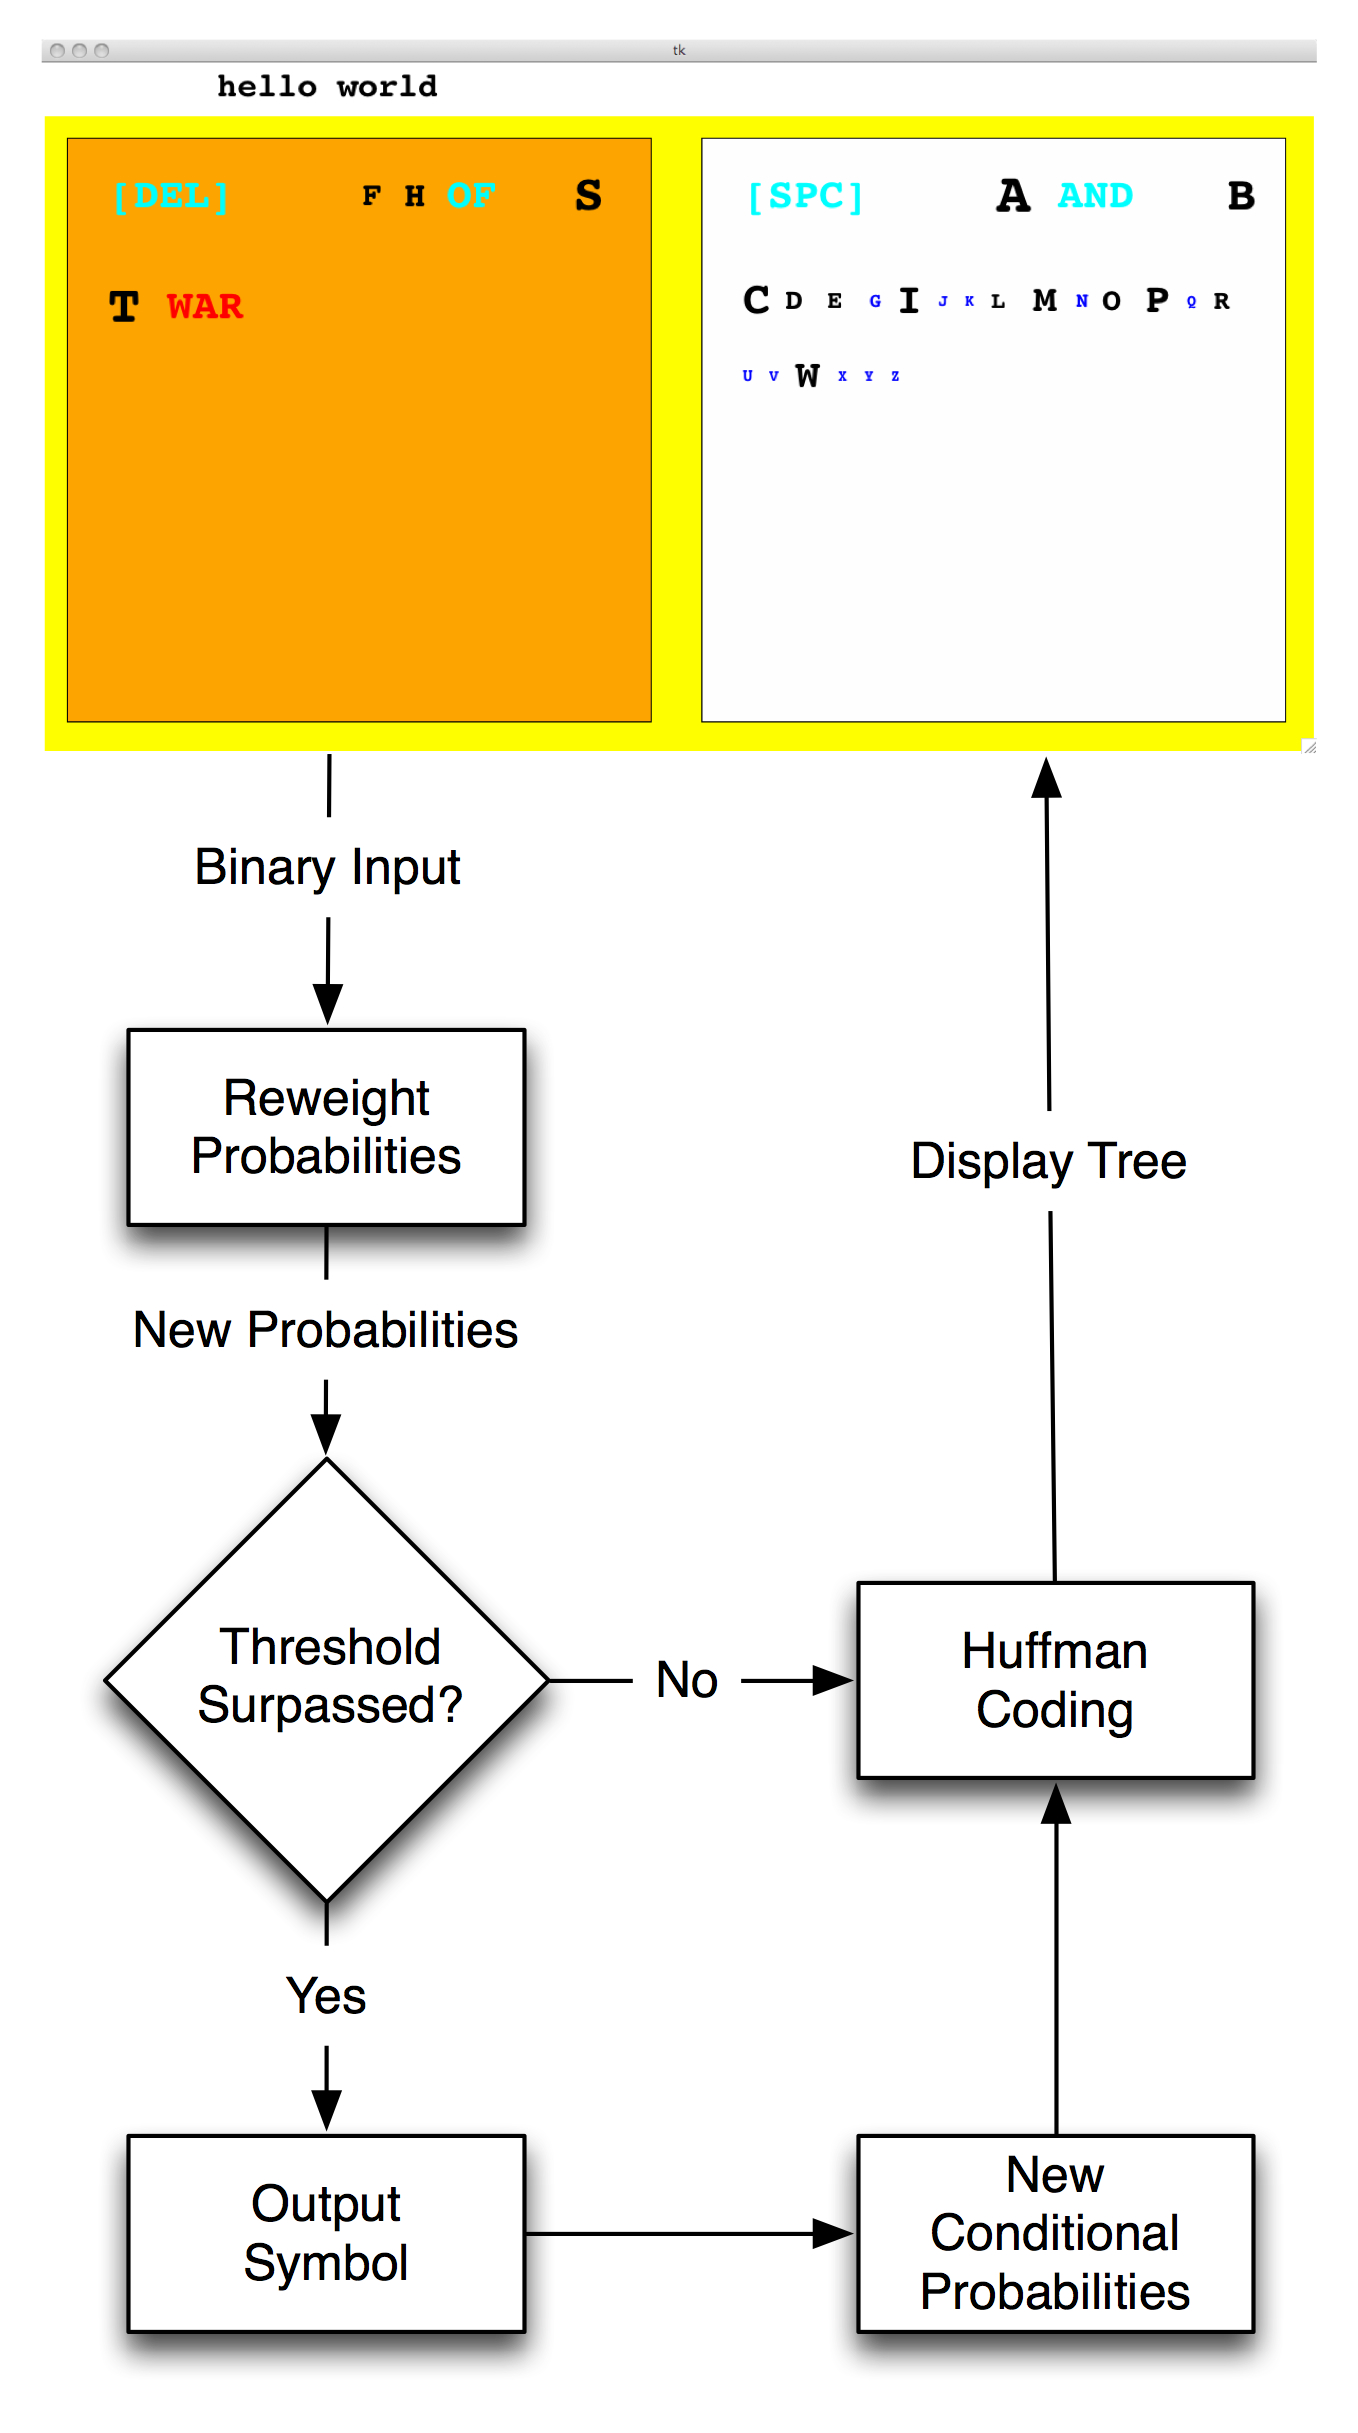
\includegraphics[scale=0.60]{fig11.jpg}
	\captionof{figure}{BinSpell FlowChart}
	\label{fig:BinFlow}
\end{center}
\end{figure}

We began by attempting to determine the most effective combination of weights and 
thresholding levels.  For this purpose, we modified BinSpell to include a routine which 
automates the typing out of text strings.  Strings are parsed  into individual word-tokens, using 
space as delimiter and words are parsed into character-tokens.  Then character-tokens are 
passed sequentially, accompanied by the word-token to which they belong, to a separate routine, which decides which box to select.  In this routine, both boxes of 
symbols are checked for the presence of the word first, followed by its accompanying 
character.  A bit corresponding to the box containing either the word or character, is sent to BinSpell's state update routine. 
Misclassification are simulated by the flipping of a bit at error-rates $0.1$, and $0.2$.  The output text is checked against the original string, each time a symbol is output.  A mismatch causes delete to be output until the output string sequence exactly matches the original string sequence from it's beginning to the length of the output string.  A count is 
kept of both the number of bits and the number of characters correctly output.  Once a phrase 
has been typed out completely without error, the number of bits sent is used to calculate a 
typing speed.  The calculated typing speeds assume 3s per bit.

This process is repeated for 5 phrases, 100 times each.  The phrases are chosen from  among 
the top 10 Google search queries, for the  U.S. on Nov. 13th, 200949.  These were: 
\begin{enumerate}
\item tony alamo 
\item harrison barnes 
\item what drives edward phase 
\item palladia 
\item we look forward to a world founded upon 
\item walmart black friday deals 
\item wizard of oz hanging 
\item water on the moon 
\item david banner 
\item bold fresh tour
\end{enumerate}

Classifier accuracies of both 80\% and 90\% were simulated.  The total number of characters 
typed for each accuracy simulation was 193.

\section{Results}

\begin{figure}[t]
\centering
\subfigure[]{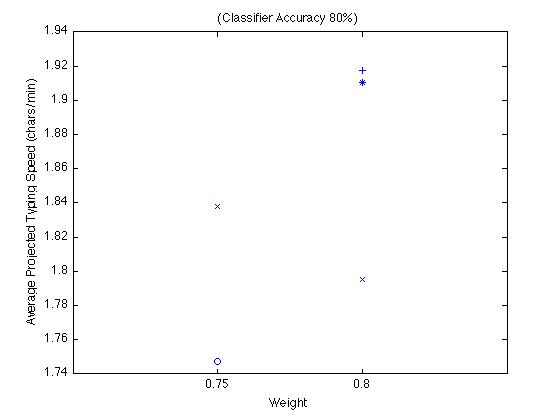
\includegraphics[width=.4\textwidth]{WeightComp_80.jpg}}
\subfigure[]{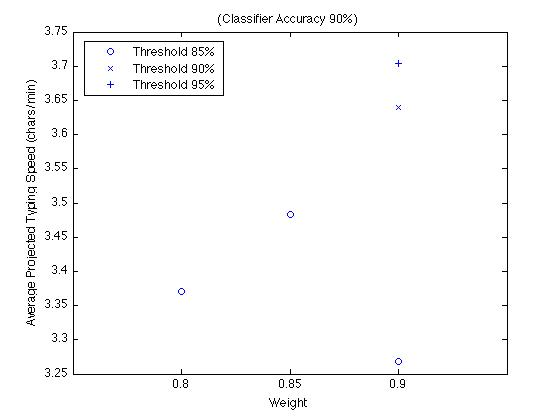
\includegraphics[width=.4\textwidth]{WeightComp_90.jpg}}
\caption{Effects of varying weight and threshold on the typing performance.}
\label{fig:WeightComp}
\end{figure}

The effects on typing speed of varying the weights and thresholds for error rates of $0.2$ and $0.1$, 
are shown in Figure~\ref{fig:WeightComp}.  On the $x$-axis are the values by which the probabilities of the symbols
in a chosen set are weighted.  The best performance simulating both error-rates was obtained 
when the weights were set to the classifier accuracy.  For both simulations, weighting by values 
less than the classifier accuracy resulted in reduced performance.   Also in both cases, 
thresholding at a value equal to the weights, significantly reduced performance.  This reduction 
is pronounced when the accuracy is 80\%.   The lowest typing speeds resulted when the weights 
were set to lower than the classifier accuracy.

\begin{figure}
\centering
\subfigure[]{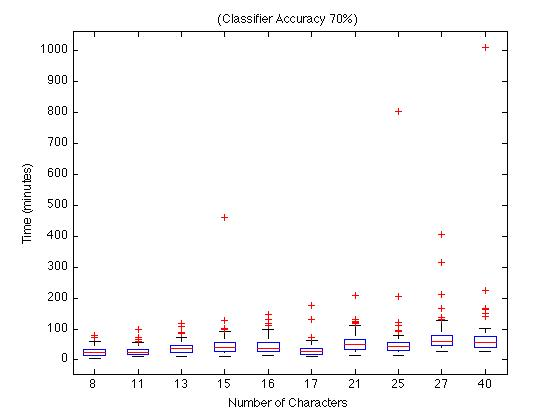
\includegraphics[width=.4\textwidth]{AutoProjTime_70.jpg}}
\subfigure[]{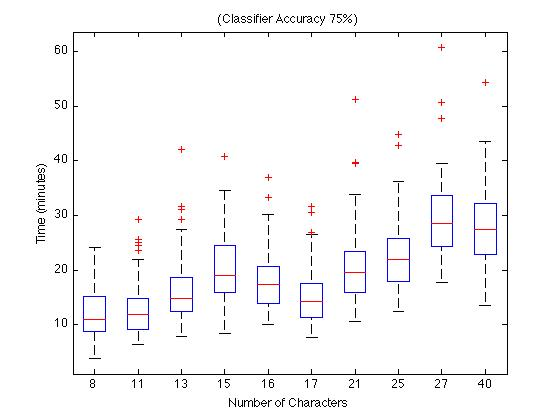
\includegraphics[width=.4\textwidth]{AutoProjTime_75.jpg}}
\subfigure[]{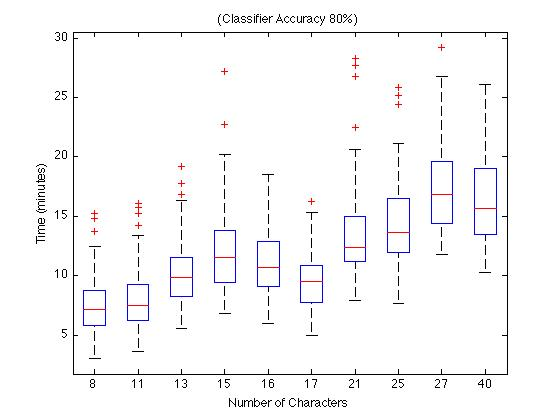
\includegraphics[width=.4\textwidth]{AutoProjTime_80.jpg}}
\subfigure[]{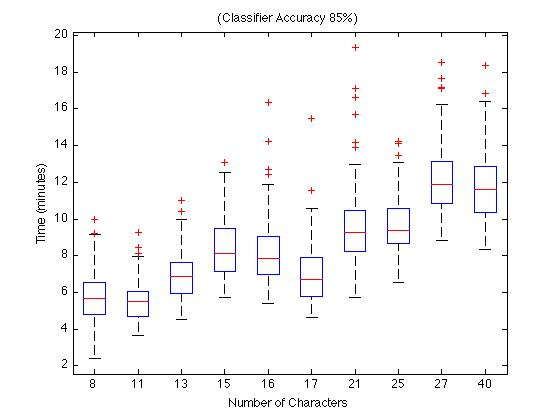
\includegraphics[width=.4\textwidth]{AutoProjTime_85.jpg}}
\subfigure[]{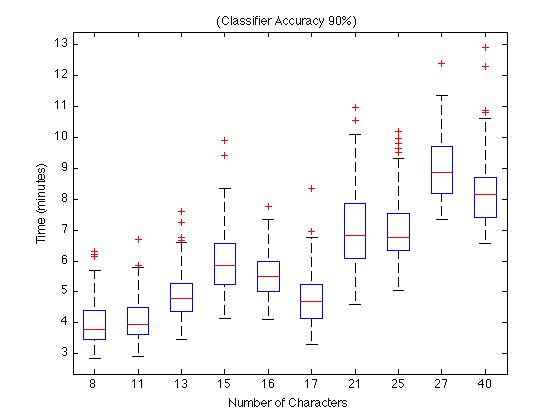
\includegraphics[width=.4\textwidth]{AutoProjTime_90.jpg}}
\caption{Time to type each phrase for varying error rates.}
\label{fig:ProjTime}
\end{figure}

Figure~\ref{fig:ProjTime} shows the number of characters versus time for each of the error rates tested. 
Predictably, the lowest time for all error-rates corresponds to the shortest sentence and the 
times vary fairly significantly with error-rates.  There is a noticeable pattern in variation among 
the error-rates.

\begin{figure}[t]
\begin{center}
	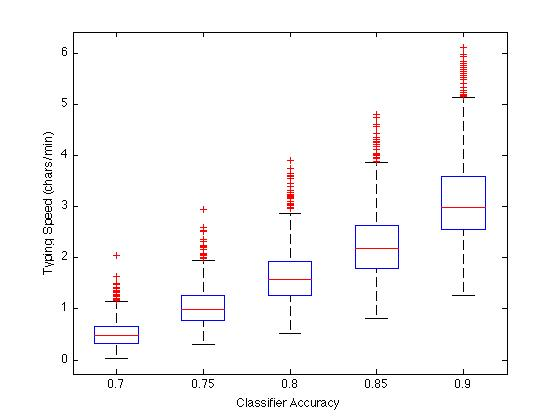
\includegraphics[scale=0.40]{ProjTypeSpeedComp.jpg}
	\captionof{figure}{Comparison of typing speeds for varying error rates.}
	\label{fig:TypeSpeed}
\end{center}
\end{figure}

\section{Discussion}

Performance in BCI controlled applications is usually reported as theoretical performance or performance with regards to an application \cite{wolpaw_braincomputer_2002}.  With regard to virtual keyboards, performance is often determined according to speed, and measured in chars/min \cite{blankertz_berlin_2006} \cite{donchin_mental_2000} \cite{wolpaw_braincomputer_2002}.  Theoretically, performance in a communication system is calculated as information transfer rate (ITR), and measured in bits/s \cite{wolpaw_braincomputer_2002}.  In this section, we discuss the performance of BinSpell with respect to both metrics.  We follow this with comparisons of BinSpell with other virtual keyboards, using the metrics they have reported.  The formula for number of bits per symbol is given as \cite{mcfarland2003brain}\cite{kelly_visual_2005}:

\begin{gather*}
	B = log_2 N + P log_2P + (1-P)log_2[\frac{(1-P)}{(N-1)}]\tag{7}\\
	BitRate = \frac{bits}{symbol} * \frac{symbols}{minute}\tag{8}
\end{gather*}
where N is the number of choices available (2 in our case), and P is the accuracy.  The bit rate is then calculated as B divided by the trial length \cite{wolpaw_braincomputer_2002}\cite{mcfarland2003brain}\cite{kelly_visual_2005}.


\subsection{Absolute Performance}

If the weighting is thought of as a ``confidence'', then the fact that setting the weights equal to 
classifier accuracy seems reasonable.  Then weighting by values lower than the classifier 
accuracy can be thought of as having less confidence in a selection, despite a less noisy 
environment.  This means the probabilities grow more ``cautiously'' than is necessary.  This 
results in an increase in the number of decisions necessary to access the symbol of choice, 
incurring a penalty on typing speed.  An increase in the number of steps to a given symbol may 
also mean more opportunity for error to occur, also reducing the typing speed.

Redundancy is a simple information theoretic tool used for the detection and correction of noise.  Thresholding is intended to introduce the redundancy intended to help deal with classifier error.  Setting the thresholding value equal to the classifier accuracy does away with the redundancy, placing too much confidence in the classifier.

The error-rate of BinSpell is calculated as the fraction of symbols output that are deletes.  For a classifier error-rate of 0.2, BinSpell's error rate is 0.1.  We calculate the actual number of bits per symbol as the number of decisions divided by the number of characters typed.  The result on average is 1.2 bits per character.  Using Equation 8, we calculate the ITR to be .03 bits/s.  

The pattern in the variation of the times in \ref{fig:ProjTime}, can be explained by 
the presence of a dictionary.  Each reduction in time corresponds to a phrase 
which contains a significant number of words found in BinSpell's dictionary.  Thus there were 
more opportunities to suggest the correct word completion, and the number of decisions made 
to complete the phrase was reduced.  All of the words in the 40-character phrase were in the 
dictionary.  The pattern also reflects a need for higher order $n$-grams, in order to better 
discriminate between words.

\subsection{Relative Performance}

\subsubsection{Circ-O-Spell vs.\ Hex-O-Spell}

Circ-O-Spell was not the focus of this study, although it did provide us with many of the exploratory ideas which led to the development of BinSpell.  Although the symbol layout of both are very similar, Circ-O-Spell's primary advantage over Hex-O-Spell is its flexible layout.  The number of 
symbols per set is not fixed.  Thus, in the best case scenario, it may only take one bit to select a 
letter, if a single letter is in a set; in the worst case it would take 11.  The best case scenario for Hex-O-Spell is 2: one for selection 
of the set, followed by selection of the character; the worst case also being 11.  In addition, the selection element of Circ-O- 
Spell, automatically orients itself over the next most probable selection, when a circle set is chosen.  This facilitates access to the most frequently used 
characters, given the typed context.  Thus, on average, fewer bits would be required for 
communication.

\subsubsection{BinSpell vs.\ P300}

Although the number of signals evoked through the flashing rows and columns have to be averaged, the P300 virtual keyboard performs significantly better than BinSpell, in terms of typing speed.  Our increase in accuracy due to redundancy comes with a significant sacrifice in speed.  But their speed-up is obtained primarily through the reduction of errors which come from the classifier.  The speller itself is not designed to handle a noisy environment, and thus would fare worse in performance given our limitations.

\subsubsection{BinSpell vs Dasher}

Dasher's zooming interface out-performs all existing virtual keyboards (see Table 1), in terms of both bit-rate and typing speed.  But using only 0.33 bit per second to effectively control a cursor would present considerable challenge to the user.  Addition of an extremely 
noisy environment would make the cursor unmanageable, as Dasher was written primarily for relatively noise-free input. As there is no method of compensating for erroneous cursor movement due to classifier error, use of Dasher given $0.33$ bits/s, and a high error-rate, would result in significantly reduced performance.

\subsubsection{BinSpell vs Hex-O-Spell}

Similarly, control of Hex-O-Spell's growing selection arrow, requires a continuous control process which would be difficult to impractical if that control was attempted in the presence of high error-rate.  Additionally, 
because Hex-O-Spell is designed for binary input, the selection element 
can only rotate in one direction.  Thus overshooting targets due to missclassifications introduces significant penalties 
in time, due to the lengthy rotation necessary to return to the desired location \cite{blankertz_advanced}.  Thus, Hex-O-Spell performance would also display greatly reduced performance given our operating constraints.

\subsection{Design Advantages}

\begin{figure}[t]
\begin{center}
	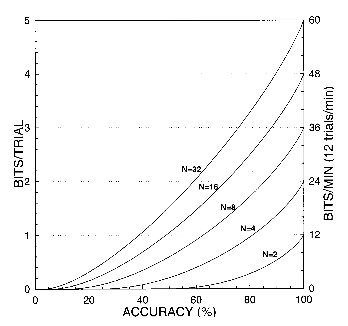
\includegraphics[scale=0.75]{fig12.jpg}
	\captionof{figure}{Information transfer rate in bits/selection and bits/min. $N$ is the number of possible choices. Shown only for accuracy greater than chance. }
	\label{fig:itrvsacc}
\end{center}
\end{figure}

\subsubsection{P300}

The P300 paradigm places limits on the user in several ways.  The P300's reliance on 
endogenous signals makes it a strictly synchronous system.  The user is forced to proceed at the 
pace of the stimuli, and does not have the option of varying the pace at which they proceed.  It 
relies on a single signal type, which may not be the best suited for the user \cite{wolpaw_braincomputer_2002}.  Also, P300's 
fixed grid approach means it is not easily modified to include alternate selection options.

In contrast, BinSpell can be extended to work with an asynchronous BCI and any type of BCI 
approach.  Its flexible, open design allows for the addition of words, phrases, and pictures.

The rapid rate of row/column intensification in the $6\times6$ matrix of the P300 speller presents a 
difficulty to users [55].  It has been suggested that involuntary eye movements in conjunction with 
the number of symbols presented, may make it difficult for a user to focus on a particular 
location on the matrix [56].  BinSpell is dynamic keyboard with a moderate presentation rate. 

The added load to the user these features present in a relatively noise-free environment, would 
be amplified in a noisy environment.  In contrast, BinSpell is designed for abbreviated 
cognitive states and does not require sustained inputs.  Although it is a dynamic keyboard, the 
symbols are presented at a moderate presentation rate.  These differences afford less frustration 
to a user communicating with BinSpell in a sub-optimal environment.

\subsubsection{Hex-O-Spell}

Parameters relating to the selection growing selection arrow employed by Hex-O-Spell, have to be tuned to the 
user for optimal performance.  Thus a new user is forced to rely on an outside expert or a 
trained user in order use Hex-O-Spell optimally.  In contrast, BinSpell requires no extra tuning, 
which makes it better suited for the general population. 

Lastly, due to it's fixed number of sets, and fixed number of options per set, Hex-O-Spell 
provides little flexibility for the addition of options such as words and phrases, while the open 
plan of BinSpell was designed with this adaptability in mind.

\subsubsection{Dasher}

Although Dasher offers the highest typing rates, there is a steep learning curve associated with 
it's control, even by conventional input methods \cite{felton2007neural}.  Additionally, BCI control of continuous 
targets often require significant training time, and often impose significant cognitive load on 
the user \cite{felton2007neural}.  Training for BinSpell, in comparison, consists of a short explanation on it's 
manipulation.  And BinSpell's lack of dependence on a continuous selection element, reduces 
the BCI training time as well.

One of the aims of research into BCI typing designs is to reduce the cognitive load on the user.  Dasher's zooming interface requires greater intense sustained attention and control for 
holding a mouse pointer steady than is required by most BCI target acquisition tasks \cite{felton2007neural}.

\section{Improving BinSpell and Future Work}

An ideal BCI keyboard given our limitation of 0.33 bits/choice would provide 0.33 bit of 
additional information each choice, with respect to the language model.  A higher order, adaptive 
language model would allow BinSpell to use bits more efficiently, while adding to a speed up in typing 
rates.  We intend to further investigate optimal policies regarding the weighting of letter with respect to words.  We also intend to use key-logging data for accurate statistics on non-alphanumeric keys.  

Keyboards with static layouts do not incur a penalty (due to scanning time) on the typing speed \cite{darragh_reactive_1992}. 
Static layouts allow users to develop strategies which facilitate their learning the keyboard, thus 
increasing the overall communication speed \cite{darragh_reactive_1992}.  We have devised a way to keep our policy of 
reordering symbols, while allowing for a static interface.  Using this approach, both sets of symbols 
would be drawn in exactly the same locations in both boxes.  The  shuffling would consist of making 
them visible or not, depending on what side of the Huffman tree they were found.  This minimally 
dynamic approach would reduce the amount of searching done by the user, and allow them to devise 
strategies associated with static interfaces. 

Despite a successful strategy for BCI-enabled communication, tests with actual severely motor-impaired subjects indicated that the P300 presented undue challenge to the user \cite{sellers_p300-based_2006}.  Thus, we also intend to test the performance of BinSpell with a BCI and motor impaired subjects in the near future.

\section{Conclusion}
BinSpell's design is based on a Huffman coded decision tree.  Selection of a character using Huffman-coded trees is given as 4.2 bits per character \cite{mackay_information_2002}.  We use a language model to predict away as much of the redundancy in language as we can, so that each choice the user makes provides the maximal amount of additional information.  Our use of language model has afforded us a decrease in information needed to select a letter, to 1.2 bits per character.    
We have presented a virtual keyboard designed for control in a severely noisy and
bandwidth-limited environment.  We borrow from natural language processing and information theory, in 
order to minimize the adverse effects of the low signal to noise ratio inherent in EEG signals, 
and the limitations of an inaccurate classifier, thus allowing communication.  Our results suggest that it is possible to enable communication rates comparable to those displayed by existing virtual keyboards, despite low classification accuracy and restricted bandwidth.

\bibliography{biblio}
\bibliographystyle{ieeepes}

\end{document}
